\chapter{Results}
\section{3D Scanning}
Several scans were carried out on the object under study, and after post-processing, a 3D model was obtained from the object.\\
A sample 3D scan carried out on the same specimen has been previously printed, which is as shown in Fig. \ref{fig:result}
\begin{figure}[!h]%
	\centering
	\subfloat[\centering Isometric View]{{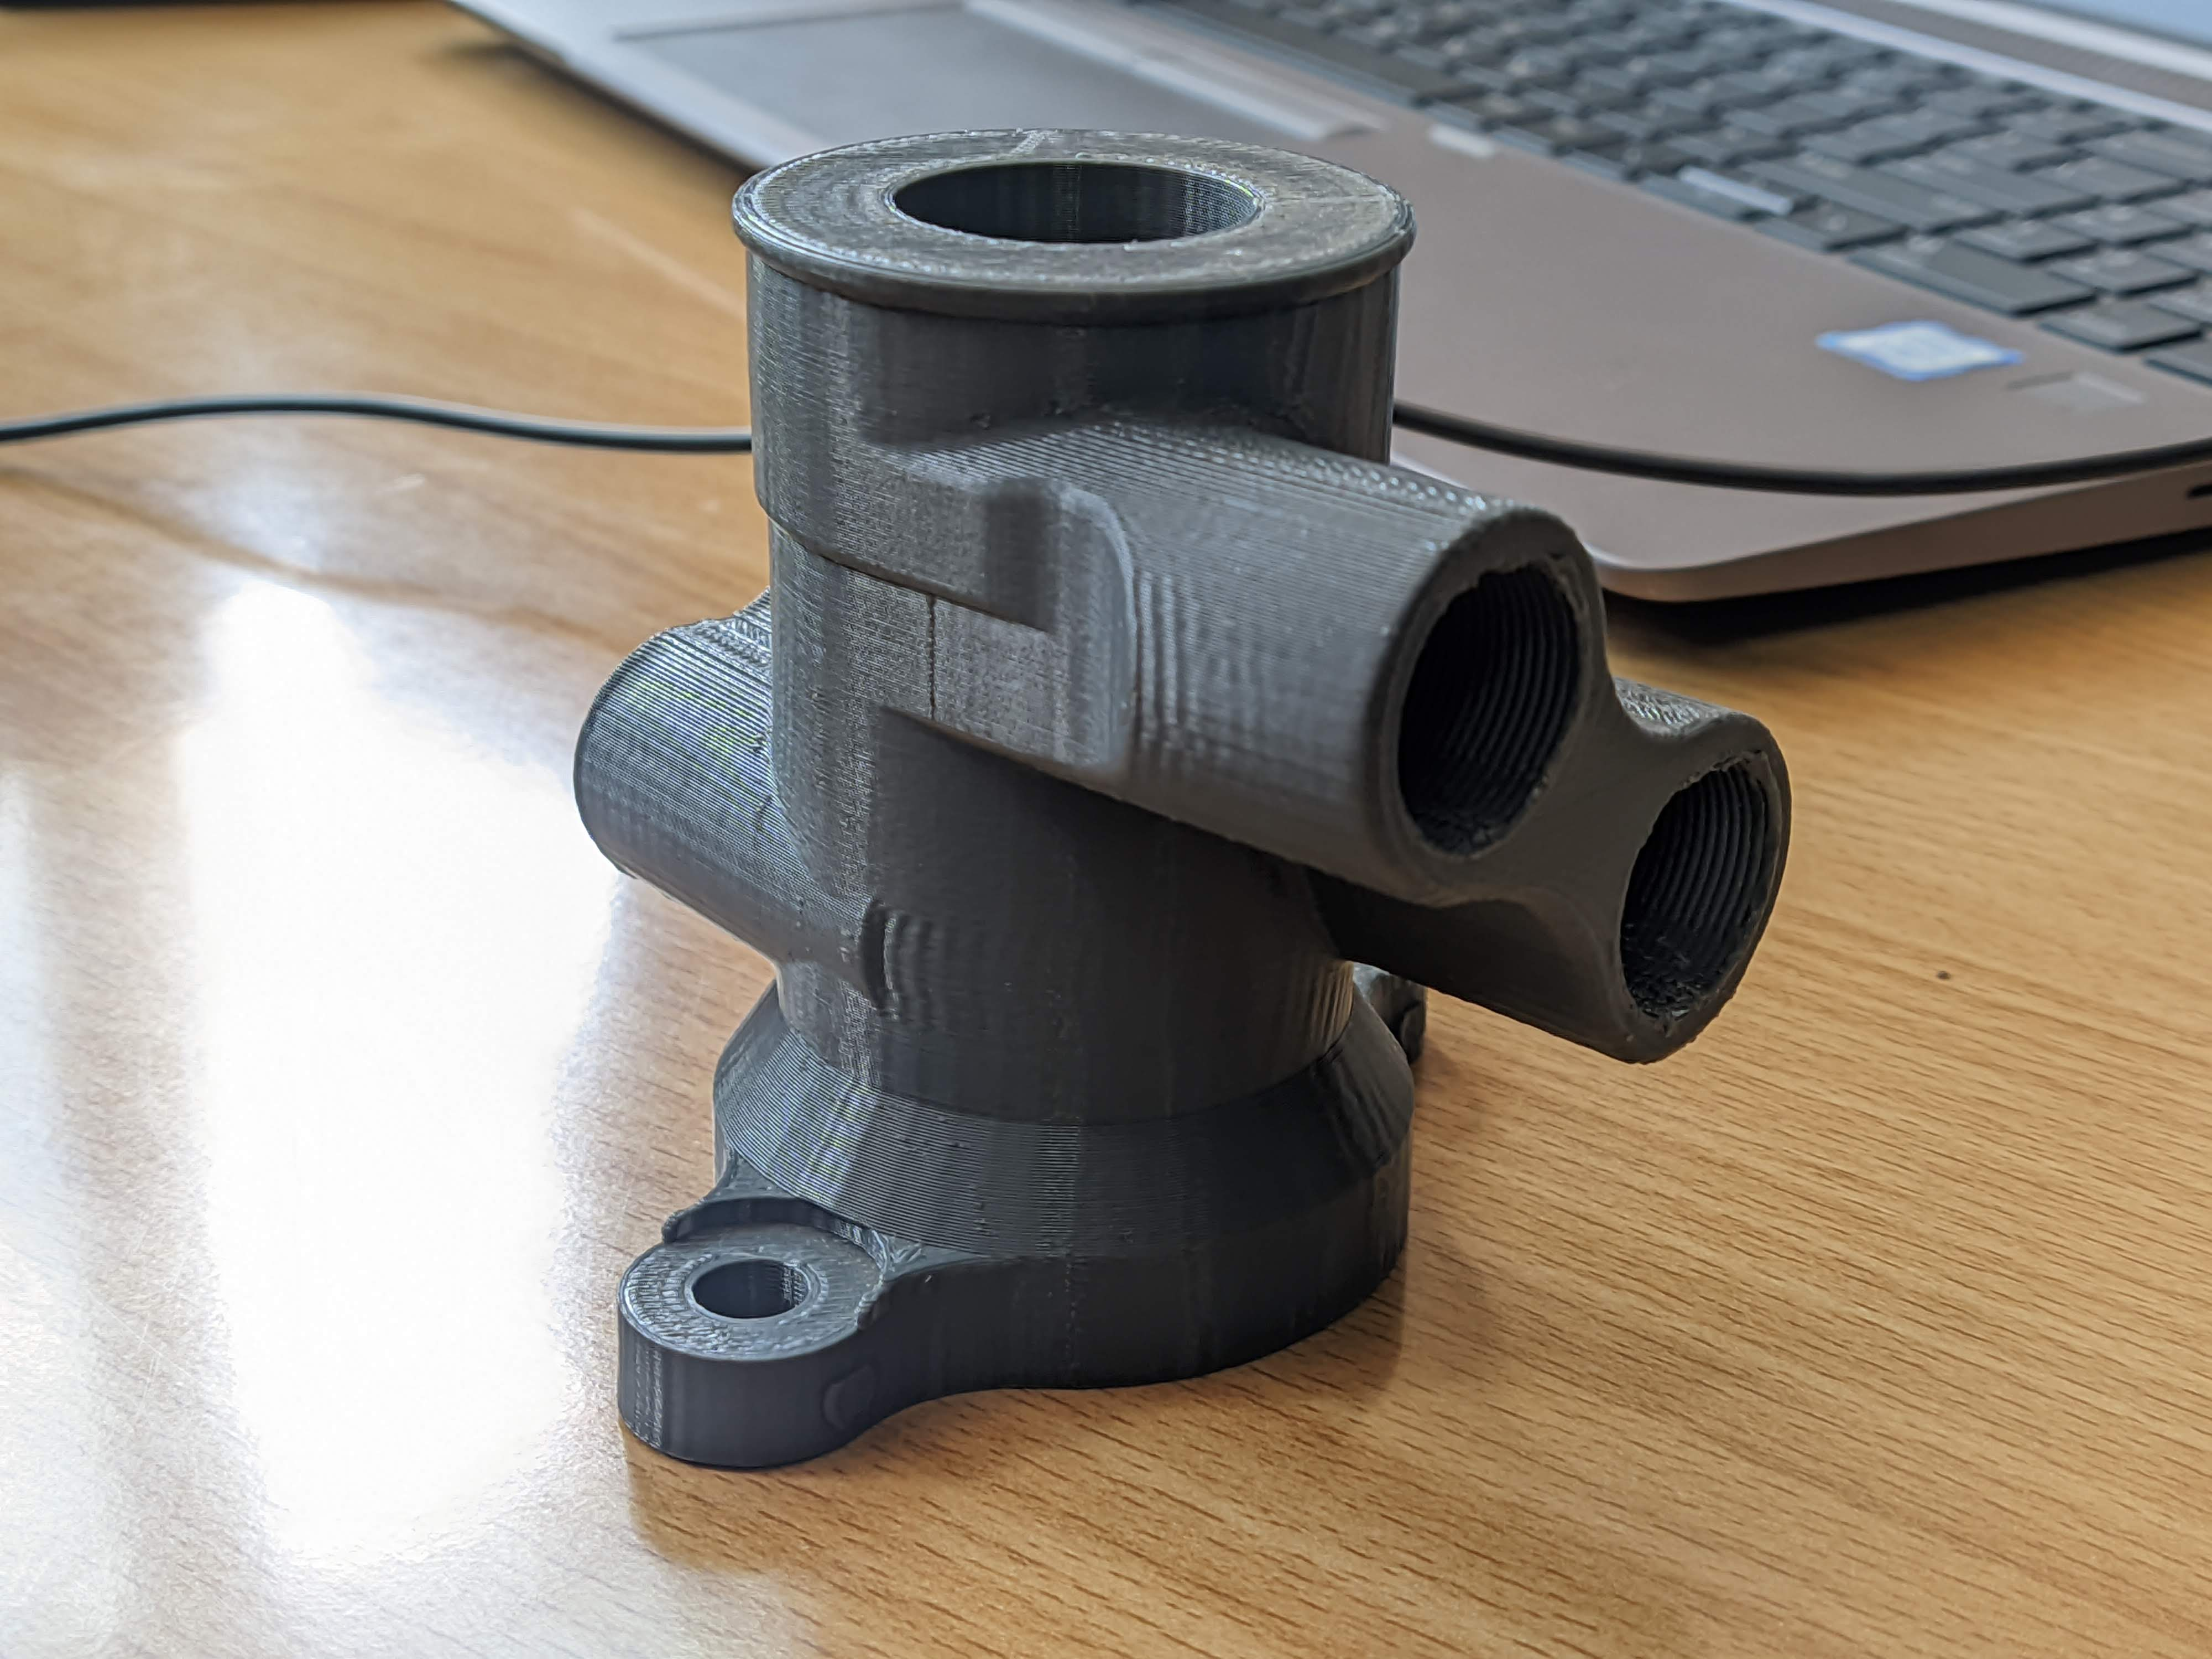
\includegraphics[width=6cm]{Figures/Result0} }}%
	\qquad
	\subfloat[\centering Top View]{{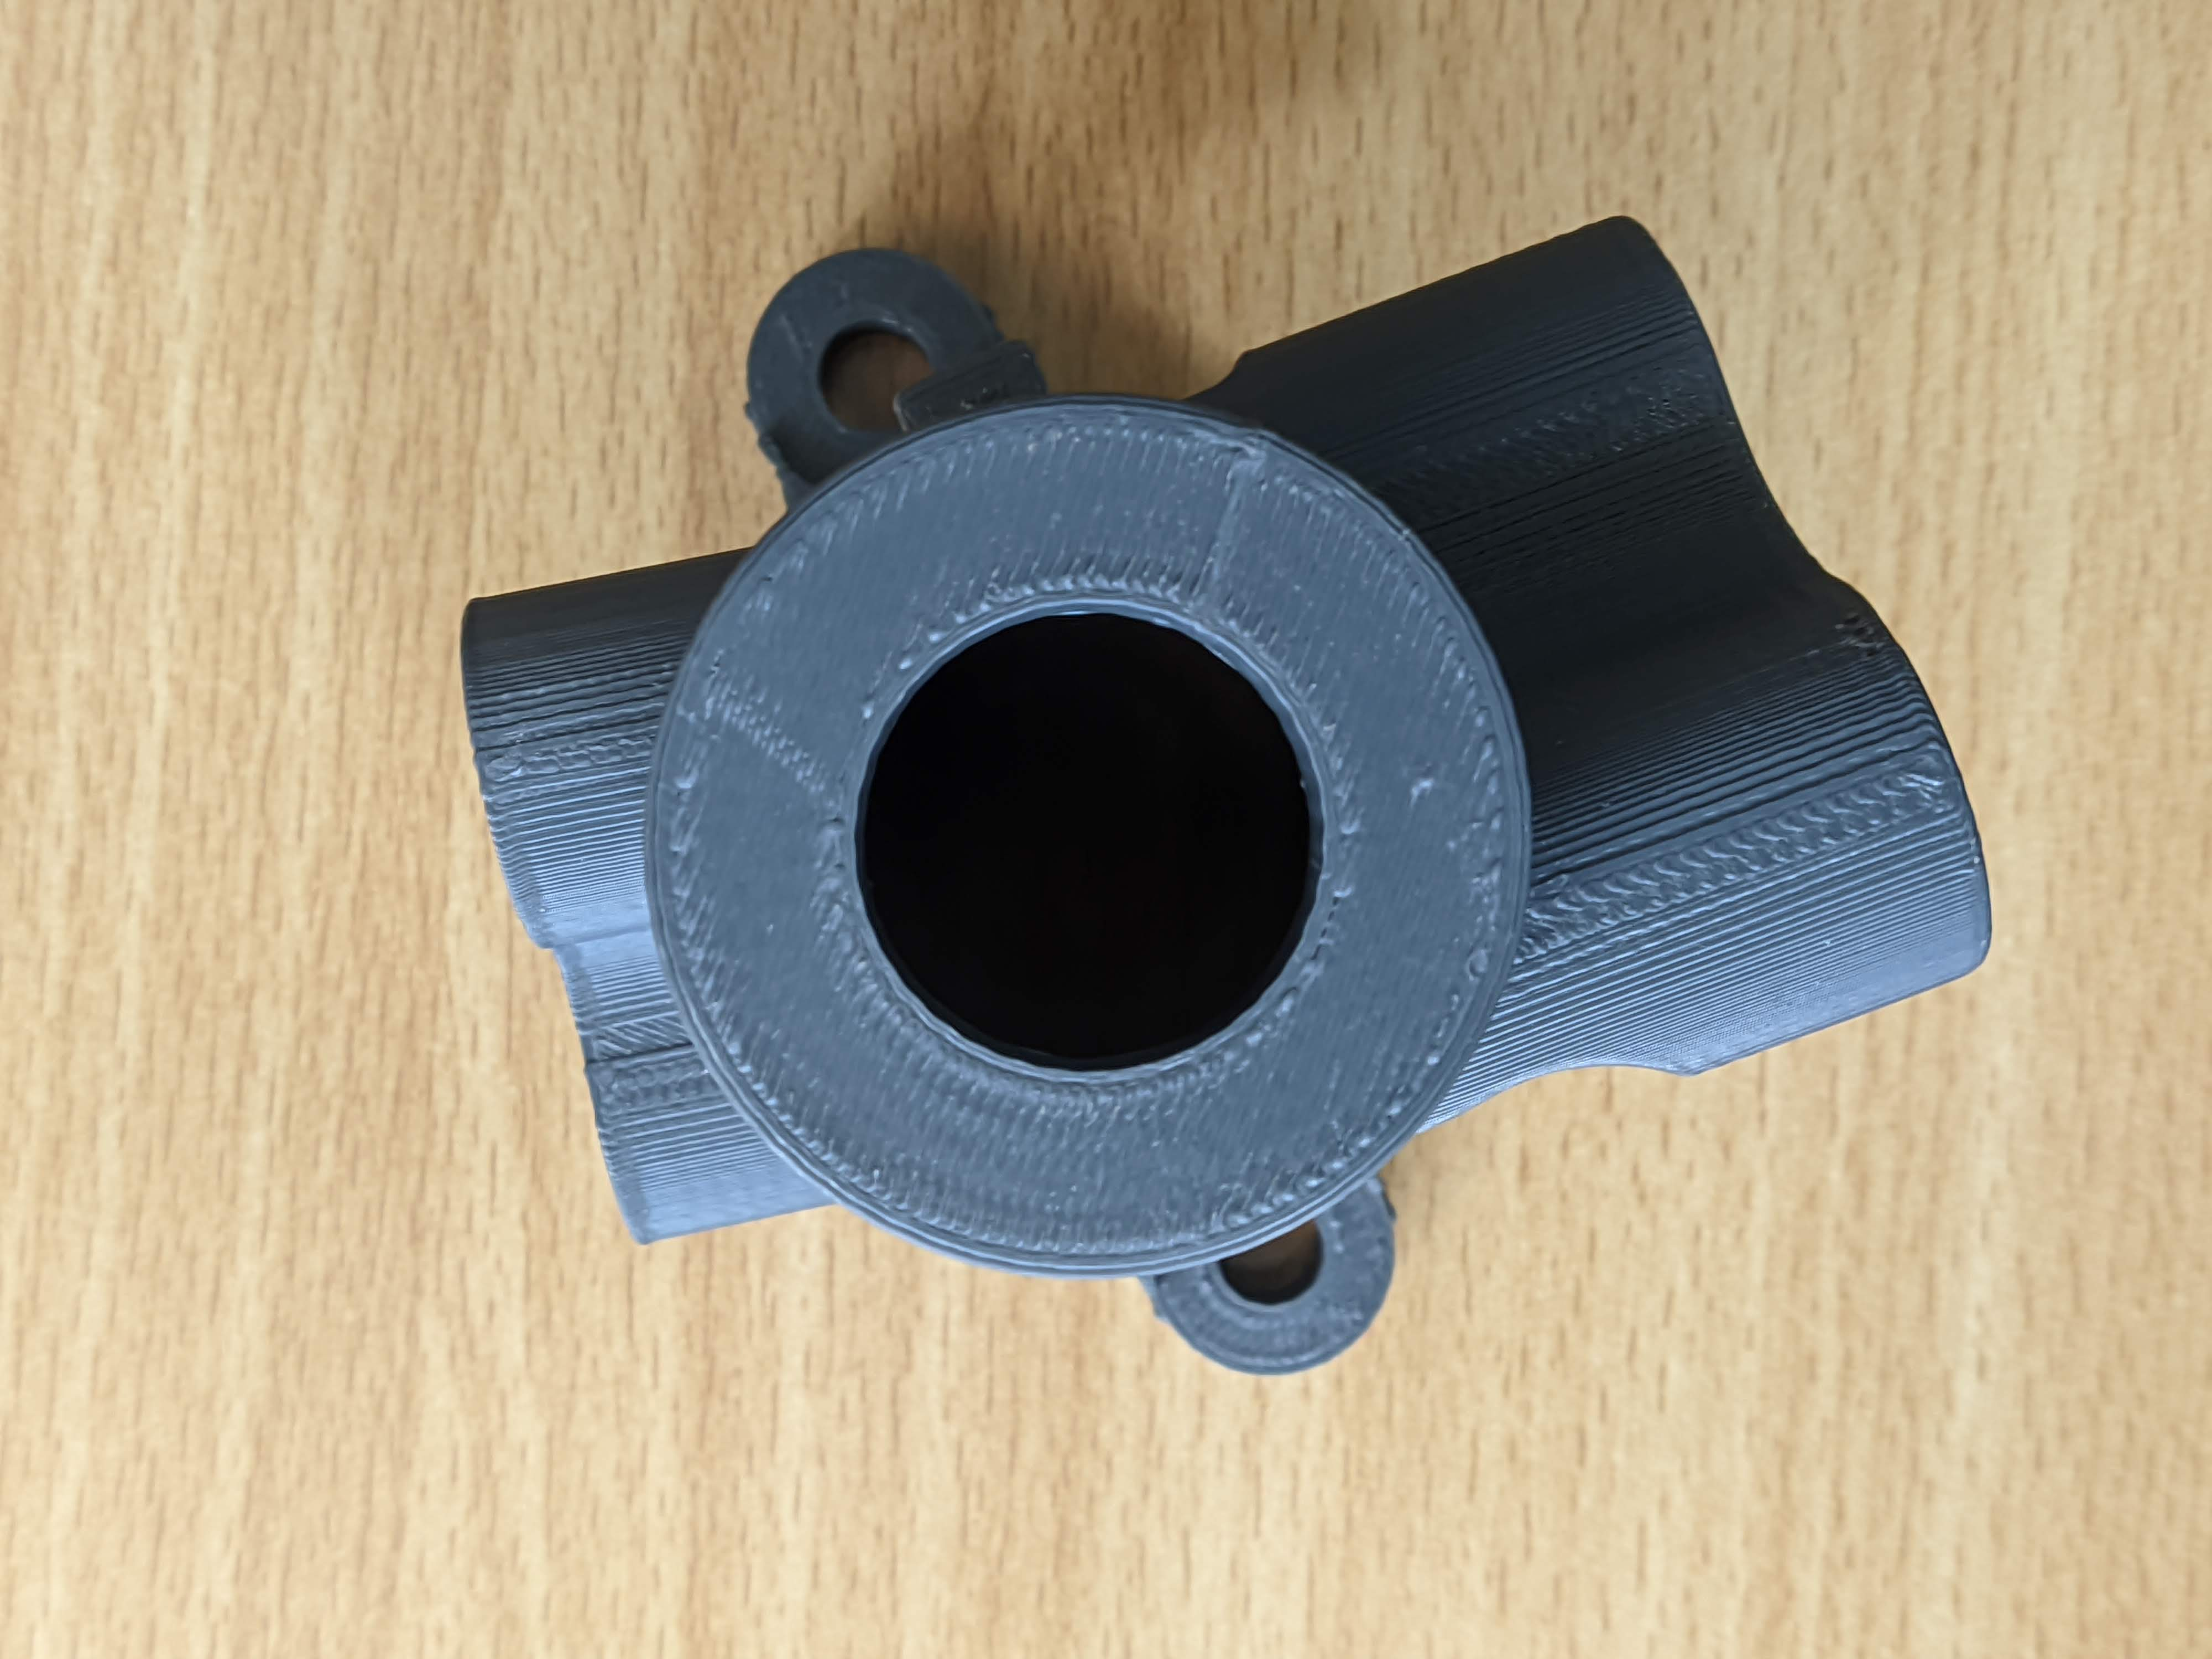
\includegraphics[width=6cm]{Figures/Result1} }}%
	\caption{Reverse-engineered 3D Print}%
	\label{fig:result}%
\end{figure}
